% Editable source for design.pdf (pdflatex design.tex; pdftoppm -png -r 150 -singlefile design.pdf design).
% The arms of the n=83 reconciliation and the exact seven-term chain from A's configuration to B's.
\documentclass[tikz,border=6pt]{standalone}
\usepackage[T1]{fontenc}
\usetikzlibrary{positioning,arrows.meta}
\begin{document}
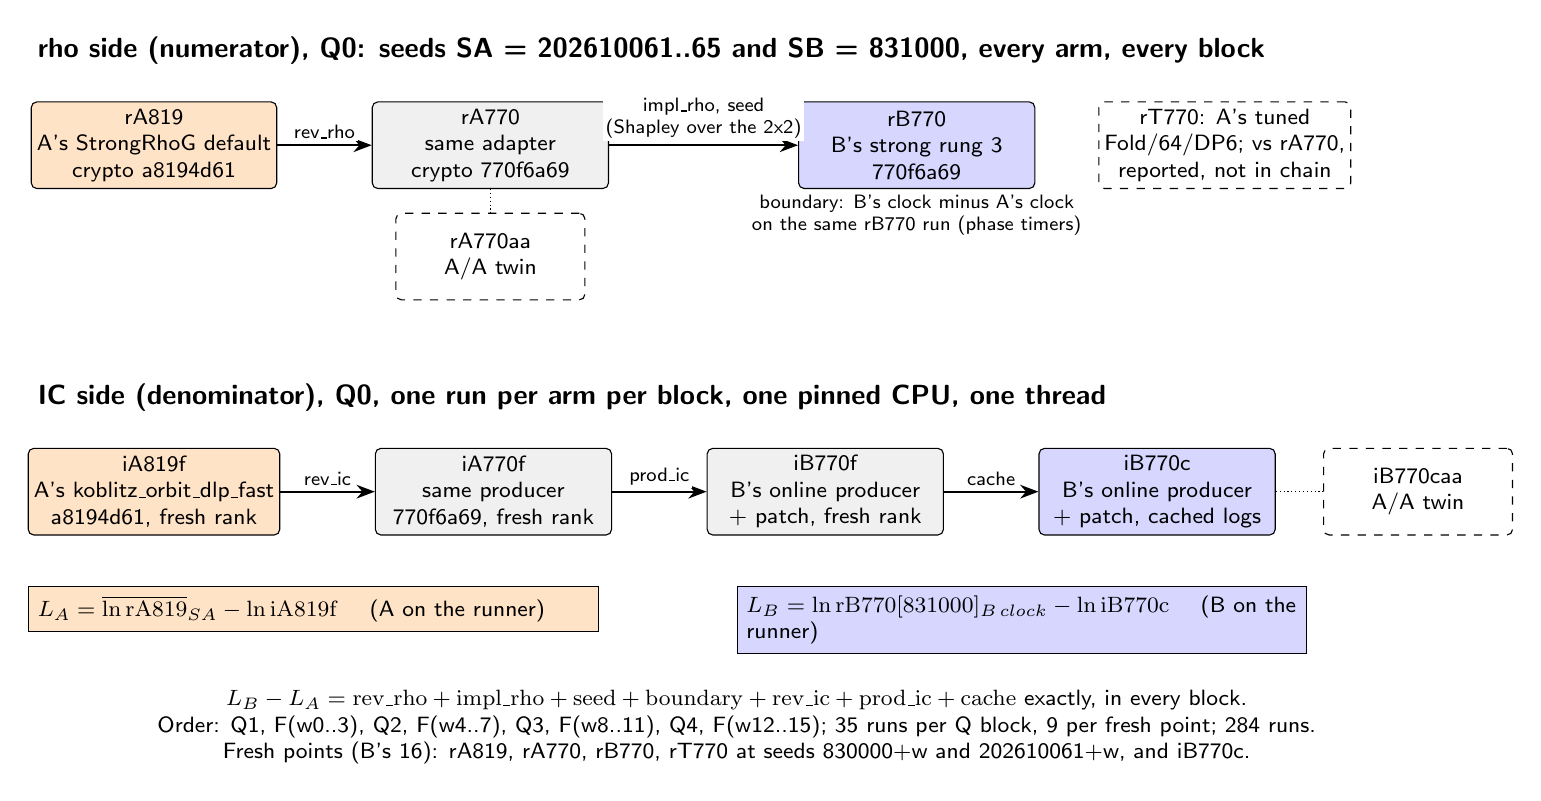
\begin{tikzpicture}[font=\sffamily\footnotesize, >=Stealth,
  arm/.style={draw,rounded corners=2pt,minimum width=30mm,minimum height=11mm,align=center,inner sep=2pt},
  a/.style={arm,fill=orange!22}, b/.style={arm,fill=blue!16}, mid/.style={arm,fill=gray!12},
  ctl/.style={arm,dashed,fill=white,minimum width=24mm},
  chainstep/.style={->,thick}, lab/.style={font=\sffamily\scriptsize,align=center,fill=white,inner sep=1pt}]
\node[font=\sffamily\bfseries,anchor=west] at (-1.6,4.4) {rho side (numerator), Q0: seeds SA = 202610061..65 and SB = 831000, every arm, every block};
\node[a] (rA819) at (0,3.2) {rA819\\A's StrongRhoG default\\crypto a8194d61};
\node[mid,right=12mm of rA819] (rA770) {rA770\\same adapter\\crypto 770f6a69};
\node[b,right=24mm of rA770] (rB770) {rB770\\B's strong rung 3\\770f6a69};
\draw[chainstep] (rA819) -- node[lab,above=1pt]{rev\_rho} (rA770);
\draw[chainstep] (rA770) -- node[lab,above=1pt]{impl\_rho, seed\\(Shapley over the 2x2)} (rB770);
\node[lab,below=1pt of rB770] (bnd) {boundary: B's clock minus A's clock\\on the same rB770 run (phase timers)};
\node[ctl,right=8mm of rB770] (rT) {rT770: A's tuned\\Fold/64/DP6; vs rA770,\\reported, not in chain};
\node[ctl,below=3mm of rA770] (aa) {rA770aa\\A/A twin};
\draw[densely dotted] (rA770) -- (aa);

\node[font=\sffamily\bfseries,anchor=west] at (-1.6,0.0) {IC side (denominator), Q0, one run per arm per block, one pinned CPU, one thread};
\node[a] (iA819) at (0,-1.2) {iA819f\\A's koblitz\_orbit\_dlp\_fast\\a8194d61, fresh rank};
\node[mid,right=12mm of iA819] (iA770) {iA770f\\same producer\\770f6a69, fresh rank};
\node[mid,right=12mm of iA770] (iBf) {iB770f\\B's online producer\\+ patch, fresh rank};
\node[b,right=12mm of iBf] (iBc) {iB770c\\B's online producer\\+ patch, cached logs};
\draw[chainstep] (iA819) -- node[lab,above=1pt]{rev\_ic} (iA770);
\draw[chainstep] (iA770) -- node[lab,above=1pt]{prod\_ic} (iBf);
\draw[chainstep] (iBf) -- node[lab,above=1pt]{cache} (iBc);
\node[ctl,right=6mm of iBc] (iaa) {iB770caa\\A/A twin};
\draw[densely dotted] (iBc) -- (iaa);
\node[draw,fill=orange!22,align=left,anchor=north west,text width=70mm] at (-1.6,-2.4)
 {$L_A = \overline{\ln \mathrm{rA819}}_{SA} - \ln \mathrm{iA819f}$ \quad (A on the runner)};
\node[draw,fill=blue!16,align=left,anchor=north west,text width=70mm] at (7.4,-2.4)
 {$L_B = \ln \mathrm{rB770}[831000]_{B\,clock} - \ln \mathrm{iB770c}$ \quad (B on the runner)};
\node[align=center,anchor=north] at (7.4,-3.6)
 {$L_B - L_A = \mathrm{rev\_rho} + \mathrm{impl\_rho} + \mathrm{seed} + \mathrm{boundary} + \mathrm{rev\_ic} + \mathrm{prod\_ic} + \mathrm{cache}$ exactly, in every block.\\
  Order: Q1, F(w0..3), Q2, F(w4..7), Q3, F(w8..11), Q4, F(w12..15); 35 runs per Q block, 9 per fresh point; 284 runs.\\
  Fresh points (B's 16): rA819, rA770, rB770, rT770 at seeds 830000+w and 202610061+w, and iB770c.};
\end{tikzpicture}
\end{document}
